% Asset ID: AS2ForcesTikZ-001
% Source: Chapter 5/7 Forces Transcript + MechYr2 Chapter 5 Friction PDF
% Related lesson section: Core Theory: Resolving a force into components
% Purpose: Show a force F resolved into F cos(theta) and F sin(theta).
\documentclass[tikz,border=8pt]{standalone}
\usepackage{amsmath}
\usetikzlibrary{arrows.meta, angles, quotes, decorations.pathmorphing}
\begin{document}
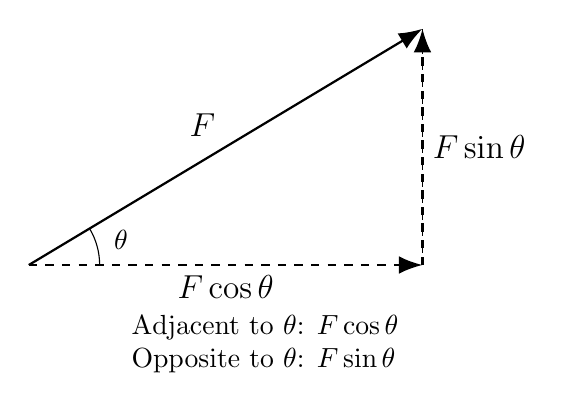
\begin{tikzpicture}[force/.style={-{Latex[length=3mm]}, thick}, comp/.style={-{Latex[length=3mm]}, thick, dashed}, label/.style={font=\large}, note/.style={font=\normalsize}]

\coordinate (O) at (0,0); \coordinate (A) at (5,0); \coordinate (B) at (5,3);
\draw[force] (O) -- (B) node[midway, above left, label] {$F$};
\draw[comp] (O) -- (A) node[midway, below, label] {$F\cos\theta$};
\draw[comp] (A) -- (B) node[midway, right, label] {$F\sin\theta$};
\draw[dashed] (B)--(A);
\pic[draw, "$\theta$", angle eccentricity=1.35, angle radius=0.9cm] {angle=A--O--B};
\node[note, align=left] at (3,-1) {Adjacent to $\theta$: $F\cos\theta$\\Opposite to $\theta$: $F\sin\theta$};
\end{tikzpicture}
\end{document}
